You emerge from the fog disoriented and half-blind. It seems that you’ve only come two or three paces, though it felt like walking a much greater distance. Behind you, the fog wall chirrs and turns an ominous, black shade. Placing a hand on it, you discover that it has solidified in your wake. There will be no turning back.\\

Something clacks off the archway by your head, and lands at your feet. An arrow. You wheel around, and your clearing vision reveals a collapsed catwalk spanning over the cell block below. On this perilous footing, two strange souls have joined forces against you: one in a guard’s uniform, the other in prisoner’s chains. A confederation of the insane.\\

The hollowed guard raises its cracked round shield into a defensive posture, and begins making its way towards you. Further across the catwalk, your former comrade nocks another arrow and takes aim.

\subsection*{Victory Condition}
Defeat both the Hollowed Guard and Hollowed Prisoner

\subsection*{Doom Events}
\begin{itemize}
\item \textbf{Round 5:} \emph{The hollowed guard ditches its shield to the ground.} Hollowed Guard will no longer commit \emph{Shield Up!} (ignore 2/5-A) and will commit \emph{Two-Handed Slash} instead of \emph{Guarded Attack} or \emph{Shield Ram}.
\item \textbf{Round 6:} \emph{It seems that the hollowed prisoner has run out of arrows.} Hollowed Prisoner no longer attempts to maintain 5 tiles distance, and will commit \emph{Knife} instead of \emph{Shortbow}.
\end{itemize}

\subsection*{Encounter Tables}
\begin{tcolorbox}
\textbf{A - Hollowed Guard}\\
\textbf{Roll:} 1D6
\begin{center}
\begin{tabular}{ L | L | L }
\multicolumn{1}{c|}{\textbf{1}} & 
\multicolumn{1}{c|}{\textbf{2-5}} & 
\multicolumn{1}{c}{\textbf{6}} \\
Move. \emph{Two-Handed Slash} &
\textbf{A:} \emph{Shield Up!} Move\newline \textbf{B:} Move. \emph{Guarded Attack}\newline \emph{This result is only exhausted after its third token} &
\textbf{A:} \emph{Sudden. Shield Ram}\newline \textbf{B:} Move. \emph{Two-Handed Slash}
\end{tabular}
\end{center}
\end{tcolorbox}

\begin{tcolorbox}
\textbf{B - Hollowed Prisoner}\\
\textbf{Roll:} 1D6
\begin{center}
\begin{tabular}{ L | L | L }
\multicolumn{1}{c|}{\textbf{1}} & 
\multicolumn{1}{c|}{\textbf{2-5}} & 
\multicolumn{1}{c}{\textbf{6}} \\
\textbf{A:} \emph{Take Aim. Shortbow}\newline
\textbf{B:} Move &
Move. \emph{Shortbow}\newline \emph{This result is only exhausted after its third token} &
\textbf{A:} \emph{Take Aim. Shortbow}\newline
\textbf{B:} Move
\end{tabular}
\end{center}
\textbf{Note:} If the Hollowed Prisoner were to commit \emph{Shortbow}, but the character is adjacent to Hollowed Prisoner, then resolve the \emph{Knife} attack instead.
\end{tcolorbox}

\begin{tcolorbox}
\textbf{Note:} Both enemies in this encounter use the same style of Encounter Table. So, instead of drawing both tables you could just use two distinct tokens on a single table.
\end{tcolorbox}

\subsection*{Enemy Sheets}
\hrule
\ \\
{\large \textbf{Hollowed Guard}}\\\\
\begin{tabular}{s s s}
\textbf{HP:} 5 & \textbf{Move:} 3\\
\textbf{P.DEF:} 1 & \textbf{PS:} 1 \\
\textbf{Shield Def:} 1 & \textbf{Shield Stab:} 4 & \textbf{Shield Dur:} -\\
\end{tabular}\\

\emph{Hollow:} This entity ignores the Charmed, Maddened, and Fear conditions.\\

\textbf{Attacks:}
\begin{itemize}
\item \emph{Two-Handed Slash} - Deal 2 Slash damage to an adjacent entity.
\item \emph{Guarded Attack} - Deal 1 Pierce damage to an adjacent entity. Do not remove \emph{Shield Up!}
\item \emph{Shield Ram} - Move 2. Deal 1 Crush damage and Knockback 1 to an adjacent entity. Do not remove \emph{Shield Up!}
\end{itemize}
\hrule
\ \\
\begin{tcolorbox}
\textbf{Note:} Remember that the Hollowed Guard has a point of \textbf{P.DEF} and \textbf{PS} in addition to a shield. See the \emph{Sinks} entry of Encounter Concepts section in the corebook for details.
\end{tcolorbox}
\ \\
\hrule
\ \\
{\large \textbf{Hollowed Prisoner}}\\\\
\begin{tabular}{s s s}
\textbf{HP:} 4 & \multicolumn{2}{l}{\textbf{Move:} 3, keeps 5 tiles distance}\\
\end{tabular}\\

\emph{Hollow:} This entity ignores the Charmed, Maddened, and Fear conditions.\\

\textbf{Attacks:}
\begin{itemize}
\item \emph{Shortbow} - Deal 1 Pierce ranged damage to an entity that is within 2-5 tiles.
\item \emph{Take Aim} - Increase the range of \emph{Shortbow} by 2 tiles this Turn. If the \emph{Shortbow} attack is made within the original range of 5 tiles, then it deals an additional 1 Pierce damage.
\item \emph{Knife} - Deal 1 Pierce damage to an adjacent entity.
\end{itemize}
\hrule
\ \\

\subsection*{Encounter Map}
\begin{center}
\framebox{
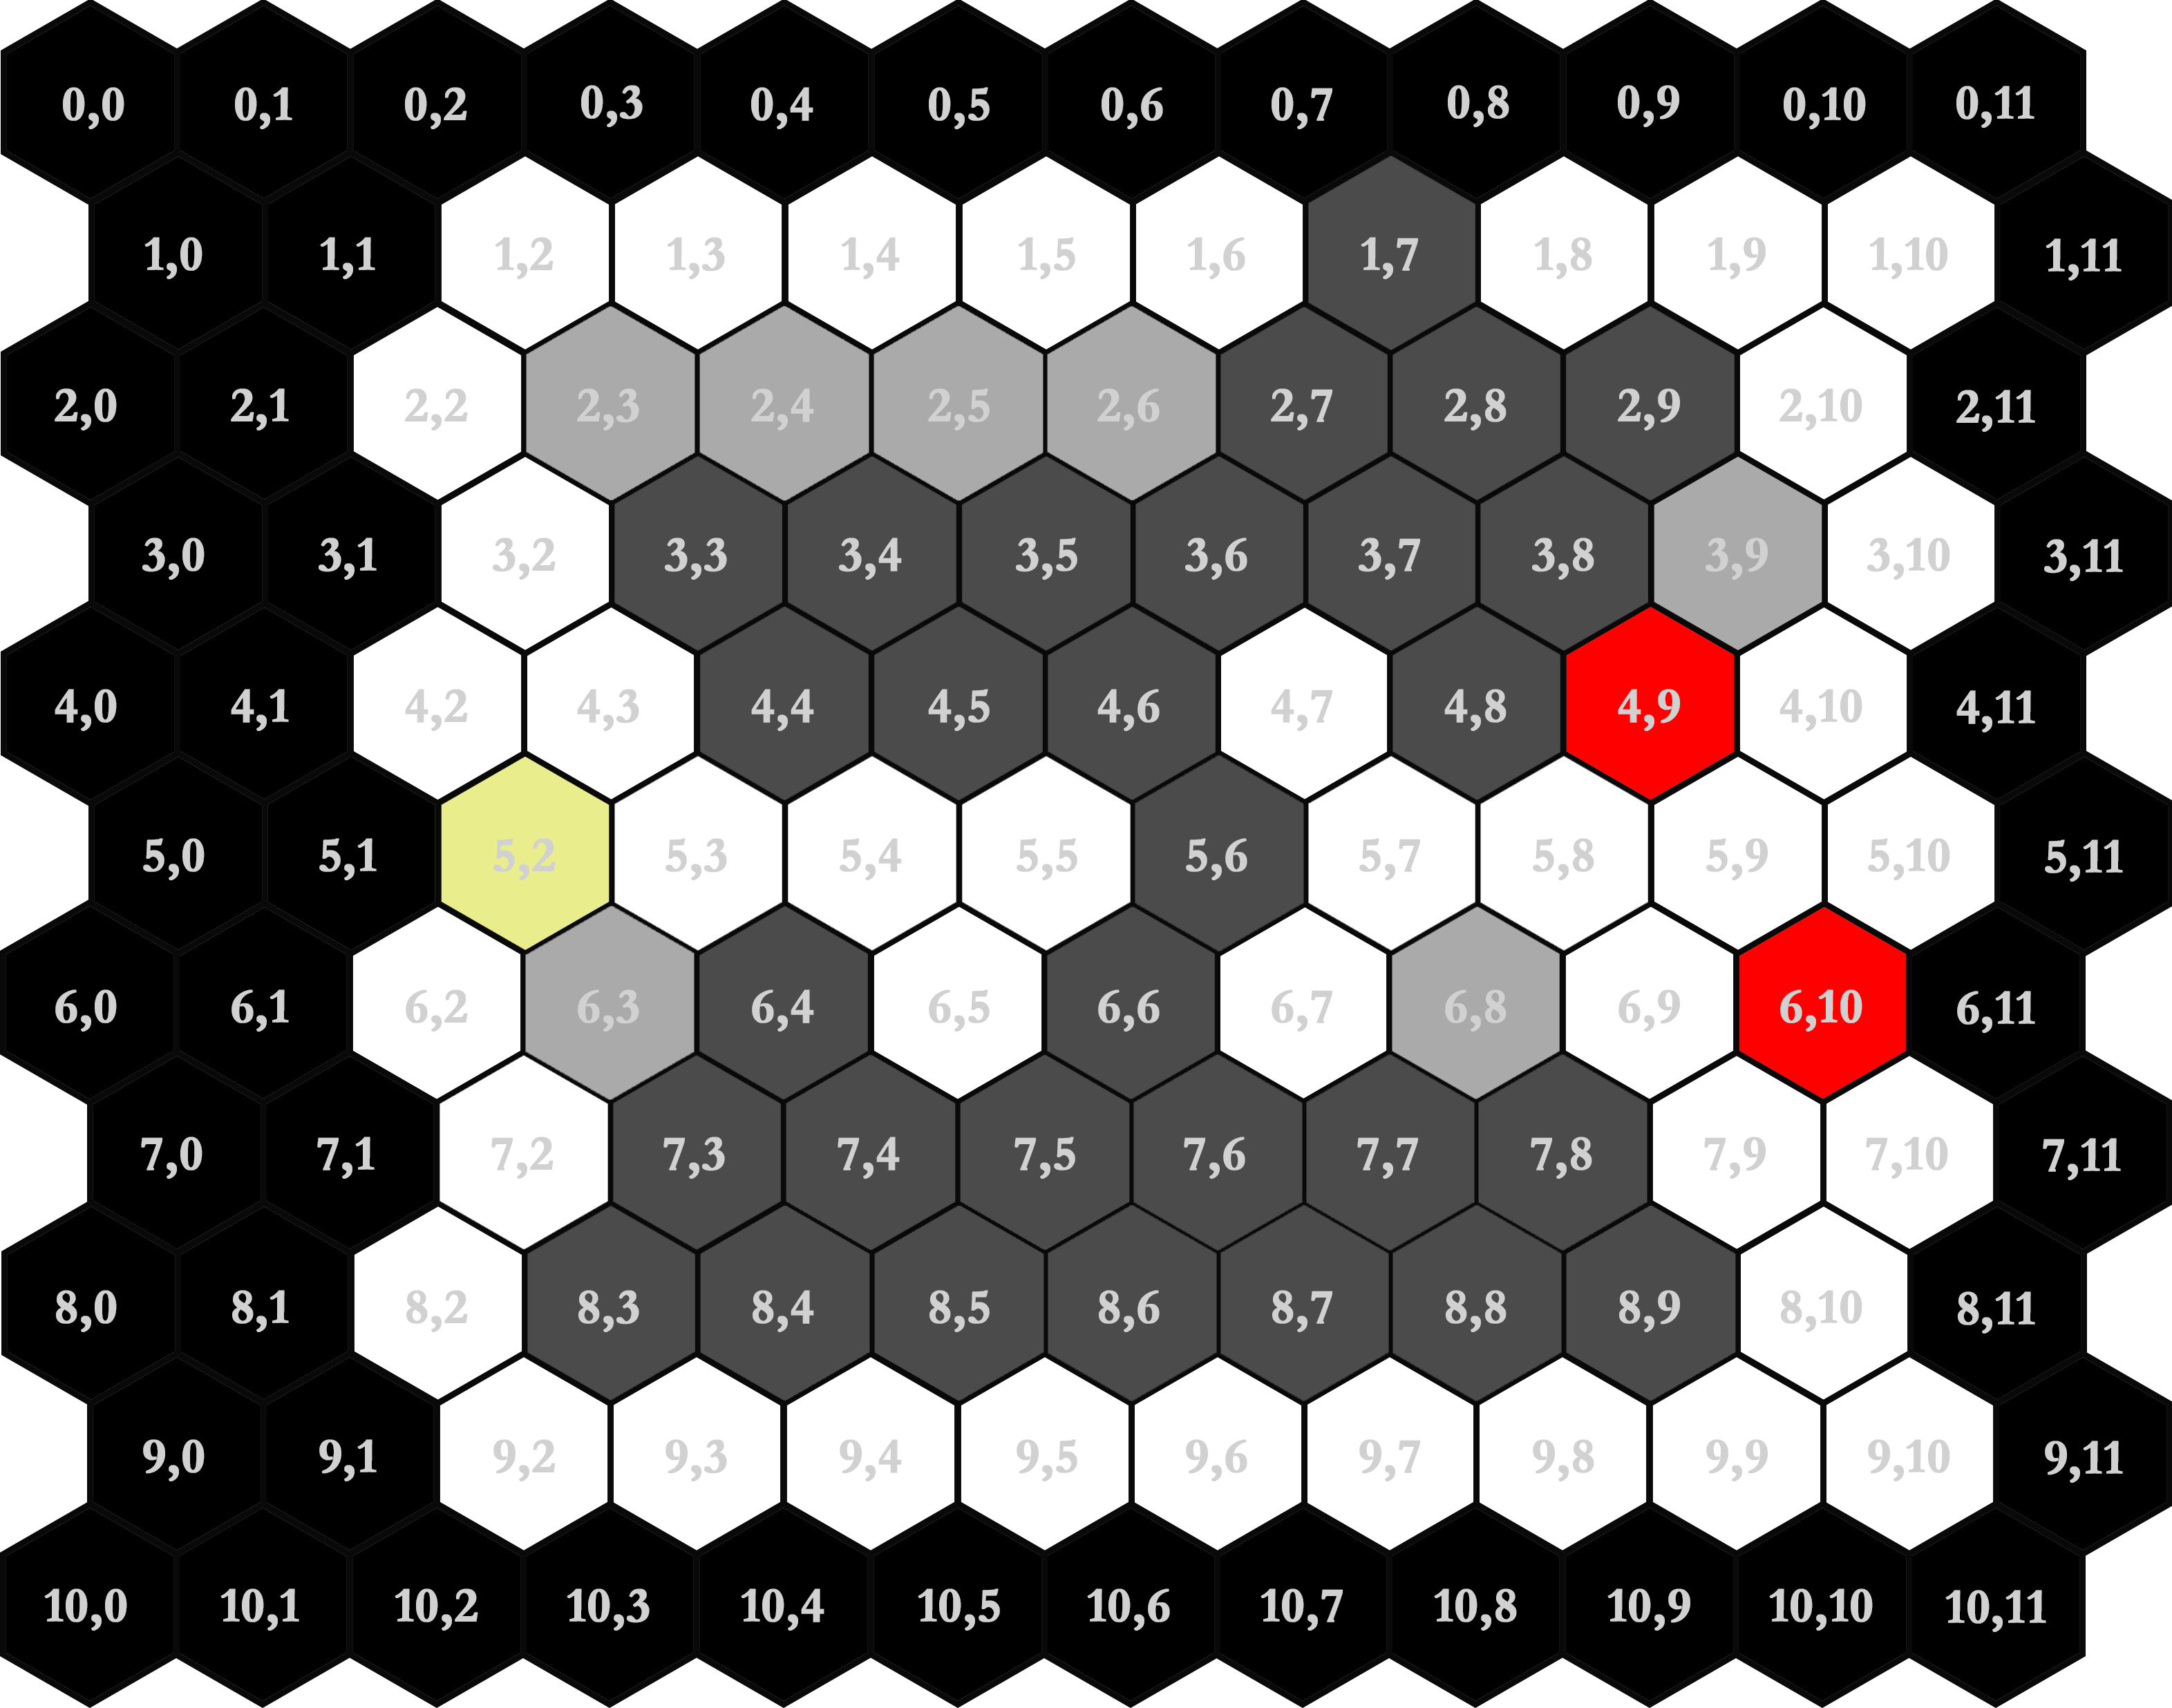
\includegraphics[width = 0.96\textwidth]{./maps/c19.png}
}
\end{center}

\subsection*{Setup Instructions}
\begin{itemize}
\item \textbf{Goldenrod:} Character Start Location.
\item \textbf{Red:} Enemy Start Locations. Place each enemy at either tile.
\item \textbf{Black:} Impassable Boundary.
\item \textbf{Dark Gray:} Pitfall. Any entity that enters this tile is defeated.
\item \textbf{Light Gray:} Half-Cover.
\end{itemize}

\begin{tcolorbox}
\textbf{Note:} Remember that the Vault action allows the character to leap over hazards and tiles of half-cover.
\end{tcolorbox}

\pagebreak

\subsection*{Victory}
The last of your opponents staggers backwards, and then drops from the catwalk. A glance over the edge reveals a lifeless corpse splayed out in a growing pool of blood. Whatever maddened thoughts brought those two together, their alliance is over now.\\

The fog has receded from this room somewhat, revealing another stairwell on the far side. Like its twin, this one is in a sorry state: collapsed into the lower levels of its spiral. Thankfully, the archway at the bottom is unobstructed--but it’s a steep drop. You won’t be returning once you make the descent.\\

>> Lost Souls (12)\\
\gain{Broken Shortsword}\\
\gain{Cracked Round Shield}\\
\gain{Shortbow}\\
\gain{Small Quiver}\\
\gain{Wooden Arrows}\\
\gain{Knife}\\
>> \turnto{c25}

\subsection*{Defeat}
Your vision blurs. You realize that you are falling--just a moment before your back hits the flagstones. Everything goes dark.\\

When you come to, it’s as if the sheer intensity of the pain had resurrected you. You blink your eyes open, and give each of your limbs a try. Nothing seems broken--just tenderized. Footsteps from above reveal that the catwalk is still being patrolled. Likely, they’ve already forgotten you were ever there. Whatever maddened thoughts have joined those two together, their alliance might just stand the test of time.\\

As for you, you’ve reached the mezzanine level of the cell block--albeit not in the way you’d planned. You pick yourself off the ground, and try to gather your bearings.\\

\emph{If the Hollowed Guard was defeated:}\\
>> Lost Soul (6)\\
\gain{Broken Shortsword}\\
\gain{Cracked Round Shield}\\

\emph{If the Hollowed Prisoner was defeated:}\\
>> Lost Soul (6)\\
\gain{Shortbow}\\
\gain{Quiver}\\
\gain{Wooden Arrows}\\
\gain{Knife}\\

>> Clear all but 1 \textbf{HP} slot of damage tokens\\
>> \turnto{c21}